\begin{enumerate}
	\item Заполните пропуски в таблице:
	\begin{figure*}[ht]
		\centering
		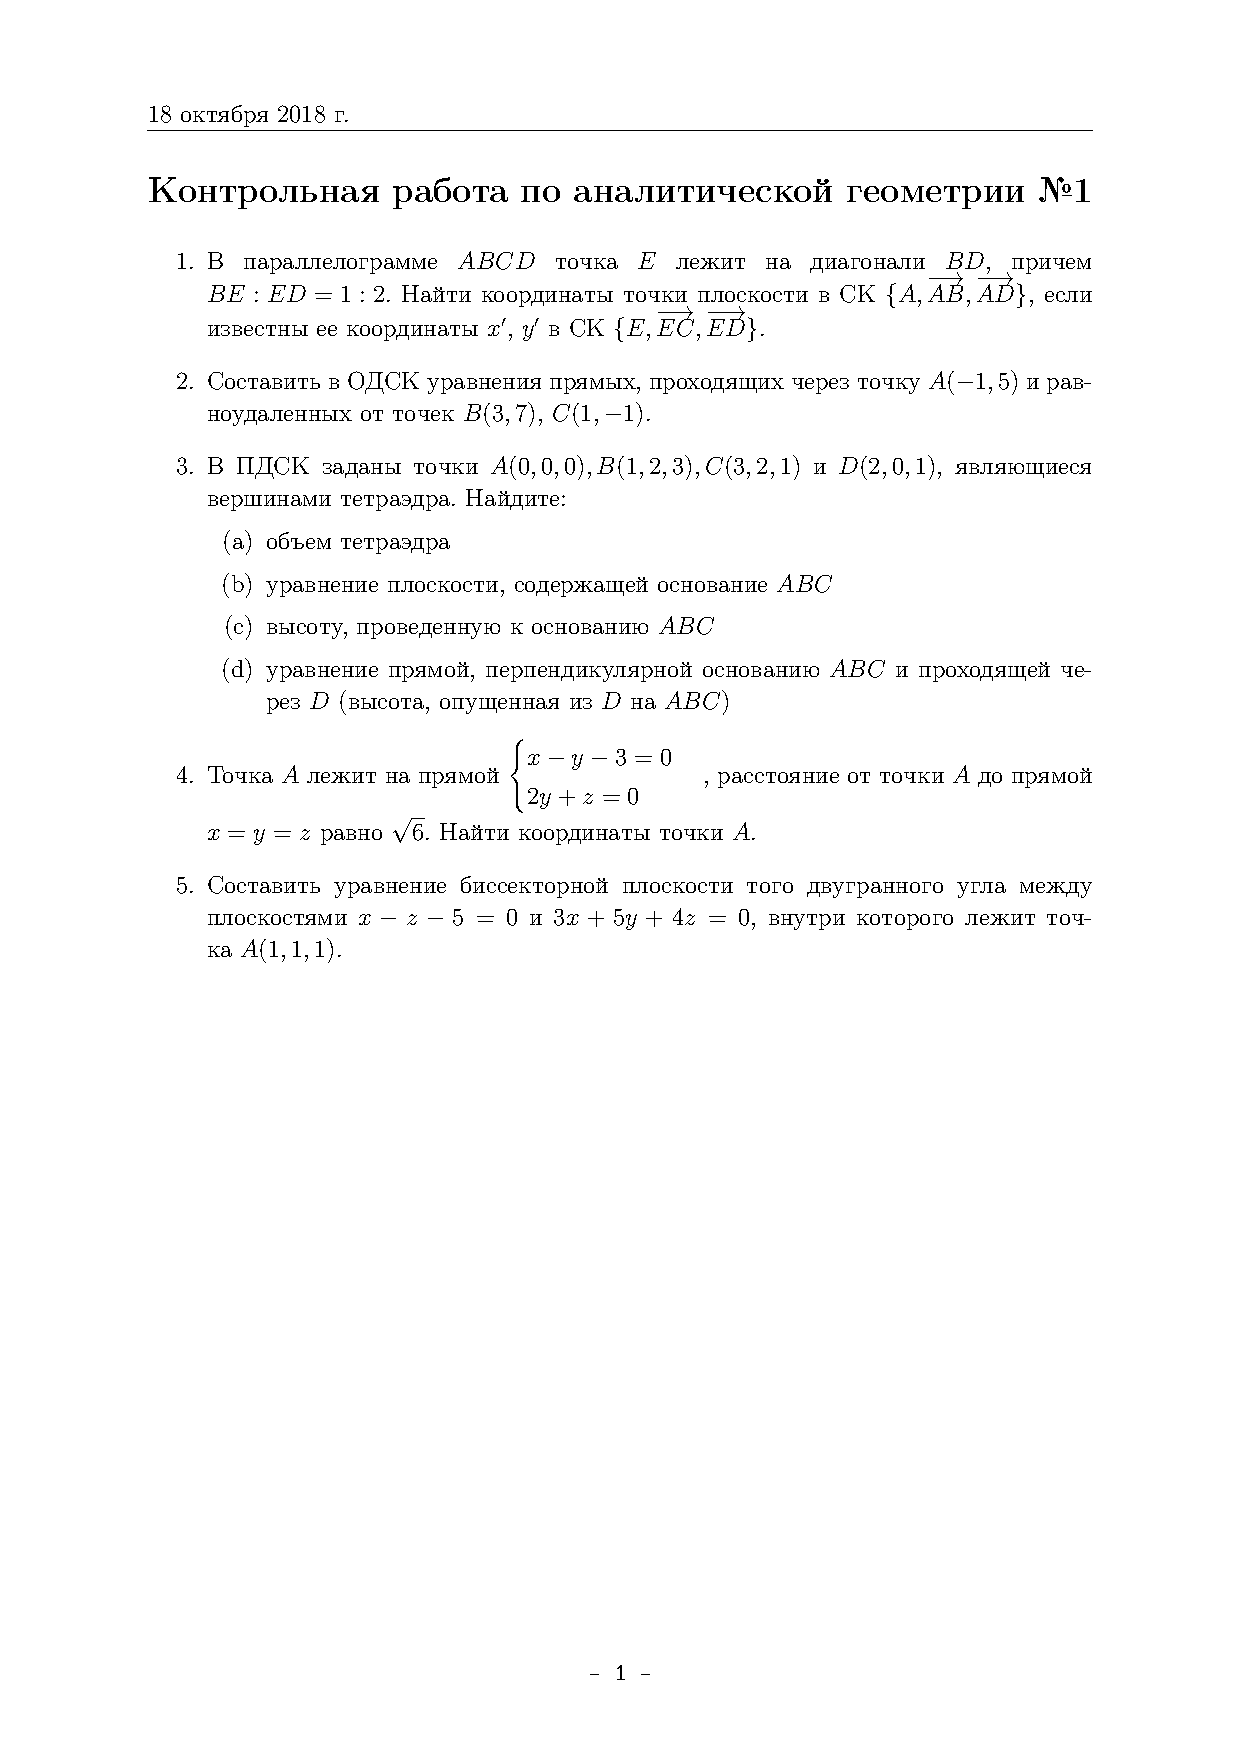
\includegraphics{1}
	\end{figure*}
	
	\item Какие из перечисленных уравнений задают некоторую поверхность вращения?
	\begin{tasks}[after-item-skip=5pt](3)
		\task $\dfrac{x^2}{2} + \dfrac{y^2}{2} + \dfrac{z^2}{3} = 1$
		\task $\dfrac{x^2}{2} - \dfrac{y^2}{2} = 2z$
		\task $\dfrac{x^2}{2} + \dfrac{y^2}{2} = 2z$
		\task $\dfrac{x^2}{4} + \dfrac{y^2}{3} - \dfrac{z^2}{3} = 1$
		\task $x^2=0$

	\end{tasks}
	
	\item Определите тип кривой $x^2 + y^2 = \lambda z^2$ при всех возможных $\lambda \in \mathbb{R}$.
	\vspace{4cm}
	\item Выберите уравнения поверхностей, содержащих прямолинейные образующие:	
	\begin{tasks}[after-item-skip=5pt](3)
		\task $x^2 + \dfrac{y^2}{2} + z^2 = 1$
		\task $x^2 + \dfrac{y^2}{2} - z^2 = 1$
		\task $x^2 + \dfrac{y^2}{2} - z^2 = 0$
		\task $x^2 - \dfrac{y^2}{2} - z^2 = 1$

	\end{tasks}
	\item Запишите параметрическое уравнения прямолинейной образующей поверхности $4x^2 + y^2 = 4$, проходящей через точку $(1,\ 0,\ 7)$.

\end{enumerate}